\documentclass{article}

% Lenguaje y Fuente
\usepackage[spanish]{babel}
\usepackage[utf8x]{inputenc}
\usepackage[T1]{fontenc}
\usepackage[top=1in, bottom=1.25in, left=1.1 in, right=1.1 in]{geometry}
\usepackage{graphicx}
\usepackage{ragged2e}
\usepackage[usenames]{color}
\usepackage{multicol}

% Portada

\title{\textbf{Reporte de la Actividad 5}\\ Midiendo el Cambio Climático a Nivel Local}
\author{Luis Fernando Duarte Gonzalí \\ Universidad de Sonora \\ Física Computacional}
\date{Febrero del 2019}
\begin{document}
\maketitle

% Contenido del Reporte

\section{Introducción}
\noindent En el siguiente documento se seguirá practicando con la biblioteca Matplotlib de Python para seguir analizando datos, se mostrarán en gráficas de los cálculos obtenidos de los índices del cambio climático. Seguiremos trabajando con el documento de \textit{Leon.txt}, ahora desde el punto de vista del análisis de datos enfocado al cambio climático a nivel local.

El archivo que se utilizó fue descargado de la página del servicio meteorológico de la columna de medias y extremas diarias.

\subsection{Climate Changes Indices}
\noindent Hay un consenso general dentro de la comunidad del clima que cambia en la frecuencia o la severidad de los eventos del clima extremo que tendrían impactos profundos en la naturaleza y la sociedad. Por eso es muy importante analizar eventos extremos. El monitoreo, la detección y la atribución a los cambios extremos en el clima usualmente requieren datos de resolución diaria. De cualquier manera, la compilación, provisión y actualización de datos de resolución diaria globalmente completa y disponible es una tarea muy difícil. Esto es porque, en parte, no todos los servicios meteorológicos e hidrometeorológicos nacionales tienen la capacidad de distribuir libremente los datos diarios que colectan. Consecuentemente, el ET y su predecesor, el CCL/CLIVAR (WG) en la detección del cambio climático han coordinado un esfuerzo internacional para desarrollar, calcular, y analizado un conjunto de índices con los cuales, los países y regiones individualmente, puedan calcular esos índices.

\section{Análisis de Datos}
Los datos que contiene el archivo de \textit{Leon.txt} van desde Enero de 1961 hasta el 2016, no contiene muchas fechas o ninguna sin datos, es decir, no tiene espacios vacíos entre estos años, es por eso que elegí ésa estación. Si es que faltaran datos se podrían interpolar los datos faltantes, pero no es muy recomendable ya que es información casi "inventada" porque no sabemos qué días sí llovió o no, ya que son procesos casi aleatorios, otra técnica sería cortar los datos y no tener gráficas con espacios vacíos por falta de información.


\noindent Para comenzar, necesitamos abrir \textsc{Jupyter Lab} desde Anaconda Prompt, abriendo la carpeta creada previamente con el nombre de \textit{Actividad5}.
Una vez abierto, en python, primero se importaron las bibliotecas Pandas, Numerical Python y Matplot para generar las gráficas.

\begin{center}
    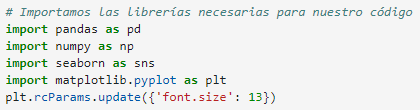
\includegraphics[scale = 0.80]{Images/Lib.png}
\end{center}

Para que python pudiera leer los archivos nulos, fue necesario reemplazar la palabra \textit{Nulo} por NaN. Además de cambiar los tipos de datos para poder trabajar con ellos.
\begin{center}
    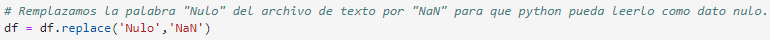
\includegraphics[scale = .74]{Images/Nan.png}
    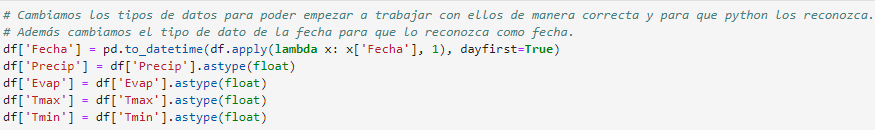
\includegraphics[scale = 0.65]{Images/Float.png}
\end{center}

\section{Resultados}
\noindent En esta sección se mostrarán las gráficas y el código utilizado para generarlas, analizando los índices del cambio climático con los datos de las dos actividades anteriores

\subsection{Número de días con heladas por año.}

\subsubsection{Código}

\begin{center}
    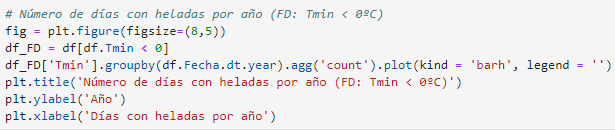
\includegraphics[scale = 0.6]{Images/Heladas.png}
\end{center}

\subsubsection{Gráfica}
\begin{center}
    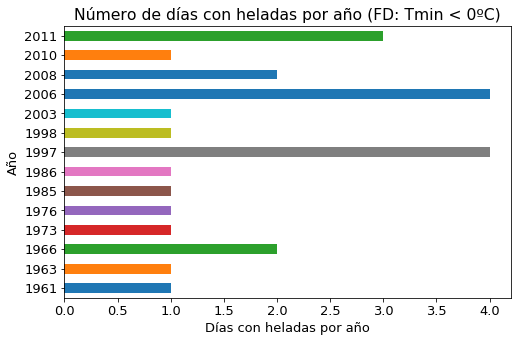
\includegraphics[scale = 0.47]{Images/GHeladas.png}
\end{center}
Se puede observar que los años con mayor número de heladas fueron 1997 y 2006, el último registrado con mayor número de heladas fue en 2011, es decir, desde el 2011 hasta el 2016 no se registraron heladas (Tmin $< 0 $°C), mientras que antes de esos años se ha visto una periodicidad de por lo menos cada 2 años ver cierto número de heladas.

\subsection{Número de Días de Verano por Año}

\subsubsection{Código}

\begin{center}
    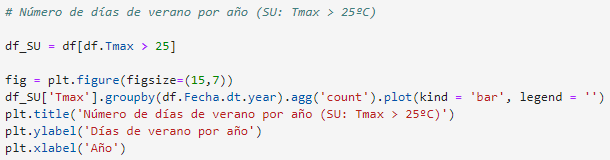
\includegraphics[scale = 0.6]{Images/Verano.png}
\end{center}
\subsubsection{Gráfica}
\begin{center}
    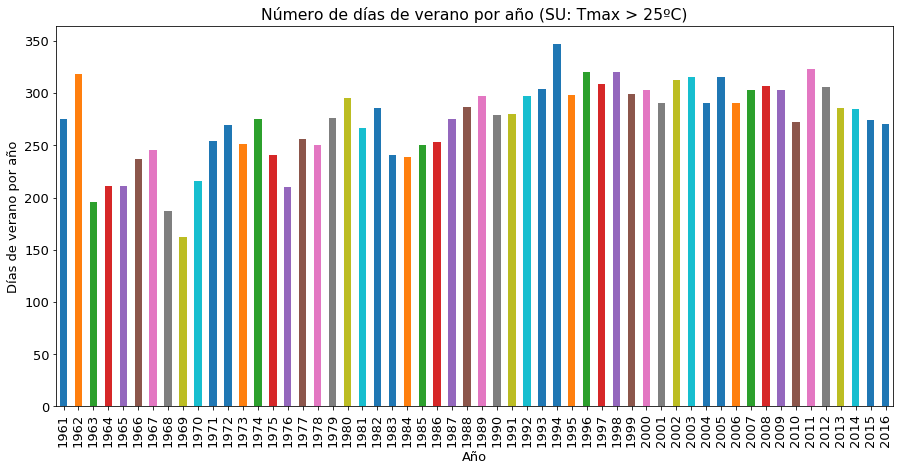
\includegraphics[width = \textwidth]{Images/GVerano.png}
\end{center}
Como se puede observar en el gráfico anterior, se ve cierta tendencia en las últimas dos décadas donde el número de días de verano ha sido mayor que 260.

\subsection{Número de Noches Tropicales por Año}

\subsubsection{Código}

\begin{center}
    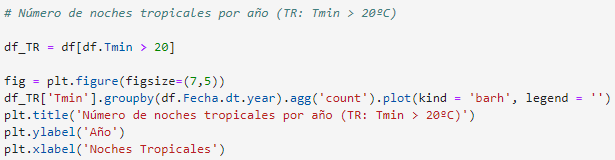
\includegraphics[scale = 0.6]{Images/Tropical.png}
\end{center}
\subsubsection{Gráfica}
\begin{center}
    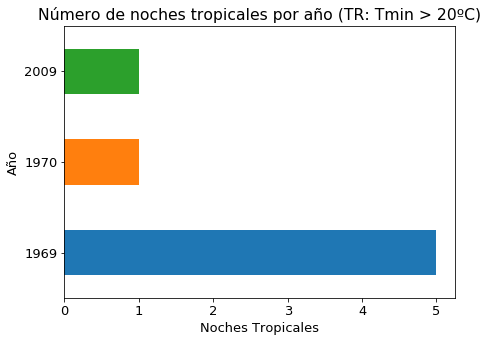
\includegraphics[scale = 0.35]{Images/GTropical.png}
\end{center}
Por otro lado podemos ver que el número de noches tropicales es muy pequeño en el periodo de tiempo (1961-2016), sólo 1969 tuvo 5 noches tropicales (Tmin $> 20$ ° C) y sólo una noche tropical en 1970 y 2009.

\subsection{La Máxima Mensual de la Temperatura Máxima}

\subsubsection{Código}

\begin{center}
    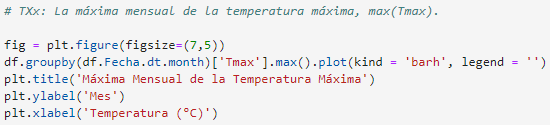
\includegraphics[scale = 0.6]{Images/maxTmax.png}
\end{center}

\subsubsection{Gráfica}

\begin{center}
    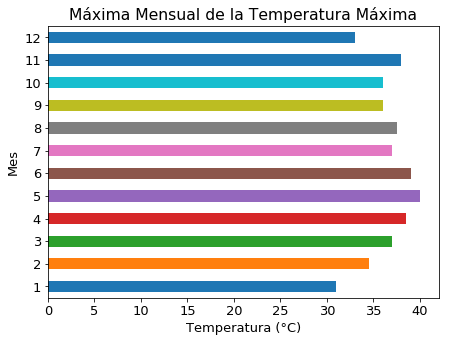
\includegraphics[scale = 0.45]{Images/GmaxTmax.png}
\end{center}
Aquí vemos la máxima mensual histórica en el periodo de tiempo antes mencionado. Donde por obvias razones vemos que el mes con mayor temperatura máxima es en Mayo, pero por falta de conocimiento no me fue posible ubicar el año en que fue esta máxima temperatura máxima.

\subsection{La Máxima Mensual de la Temperatura Mínima}

\subsubsection{Código}

\begin{center}
    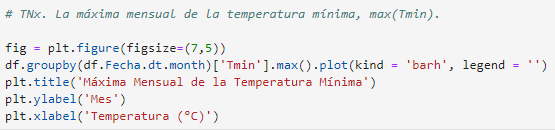
\includegraphics[scale = 0.6]{Images/maxTmin.png}
\end{center}

\subsubsection{Gráfica}

\begin{center}
    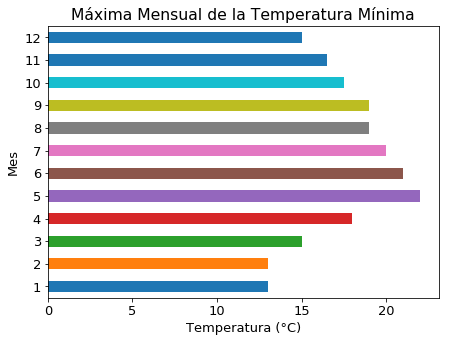
\includegraphics[scale = 0.46 ]{Images/GmaxTmin.png}
\end{center}

Aquí podemos observar de nuevo que el mes con récord histórico en la máxima temperatura mínima es mayo, igual, no se puede mostrar el año que tuvo el récord.

\subsection{El Mínimo Mensual de la Temperatura Máxima}
\subsubsection{Código}
\begin{center}
    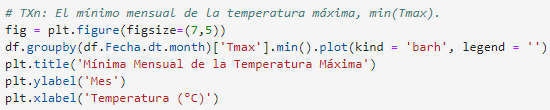
\includegraphics[scale = 0.6]{Images/minTmax.png}
\end{center}
\subsubsection{Gráfica}
\begin{center}
    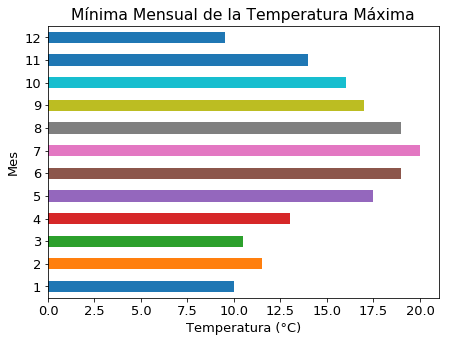
\includegraphics[scale = 0.46]{Images/GminTmax.png}
\end{center}
Por otro lado, podemos observar que la mínima temperatura máxima se dió en entre Diciembre y Enero, que es muy lógico.

\subsection{El Mínimo Mensual de la Temperatura Mínima}

\subsubsection{Código}
\begin{center}
    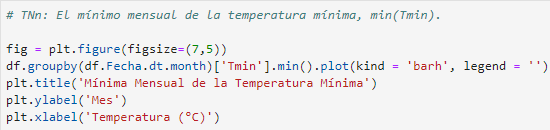
\includegraphics[scale = 0.6]{Images/minTmin.png}
\end{center}

\subsubsection{Gráfica}
\begin{center}
    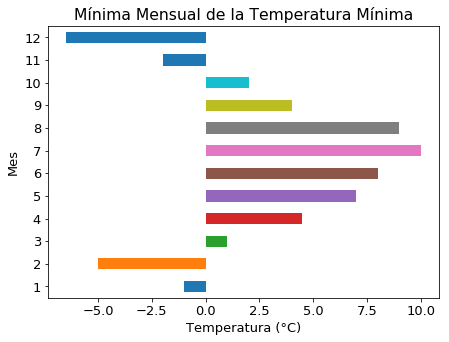
\includegraphics[scale = 0.46]{Images/GminTmin.png}
\end{center}

Igual, en Diciembre se dio la mínima temperatura mínima, alcanzando los menor que -5.0 °C.

\subsection{El Promedio Mensual de la Diferencia de Temperaturas}
\subsubsection{Código}
\begin{center}
    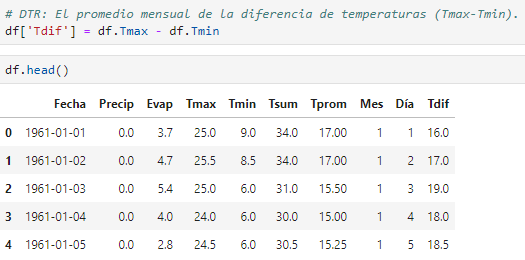
\includegraphics[scale = 0.56]{Images/TDif.png}
    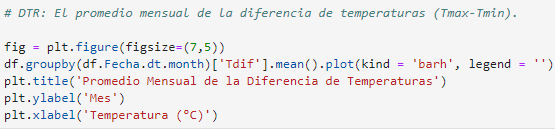
\includegraphics[scale = 0.54]{Images/TDif2.png}
\end{center}
En este caso, cree otra columna que nos mostrara la diferencia entre la temperatura mínima y máxima diaria, para poder después hacer el código que nos genere la siguiente gráfica.

\subsubsection{Gráfica}
\begin{center}
    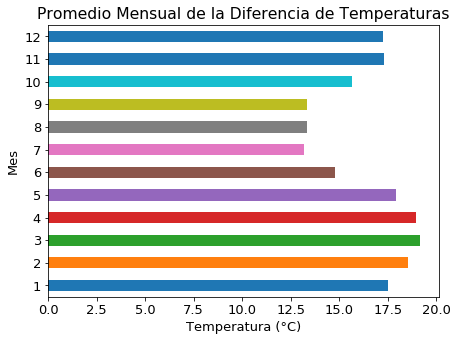
\includegraphics[scale = 0.46]{Images/GTDif.png}
\end{center}
Esta vez se muestra la gráfica de promedio mensual de la columna que se ha creado previamente para la diferencia de temperaturas mínima y máxima, donde vemos que en la ciudad de León el promedio de la diferencia de temperaturas se encuentra por debajo de los 20°C todo el año.

\subsection{Precipitación Diaria Máxima Mensual en 1 Día.}
\subsubsection{Código}
\begin{center}
    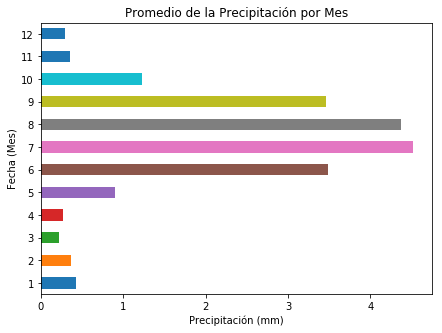
\includegraphics[scale = 0.6]{Images/Precip.png}
\end{center}
\subsubsection{Gráfica}
\begin{center}
    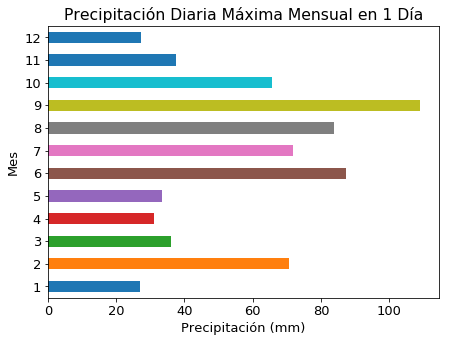
\includegraphics[scale = 0.6]{Images/GPrecip.png}
\end{center}
Ahora observamos la precipitación máxima en un solo día históricamente, donde vemos que el récord se encuentra en el mes de Septiembre, pero otra vez no pude visualizar el año en que se dio ésta máxima.

\subsection{Número de Días en un Año con Precipitación Mayor Igual a 1mm.}

\subsubsection{Código}
\begin{center}
    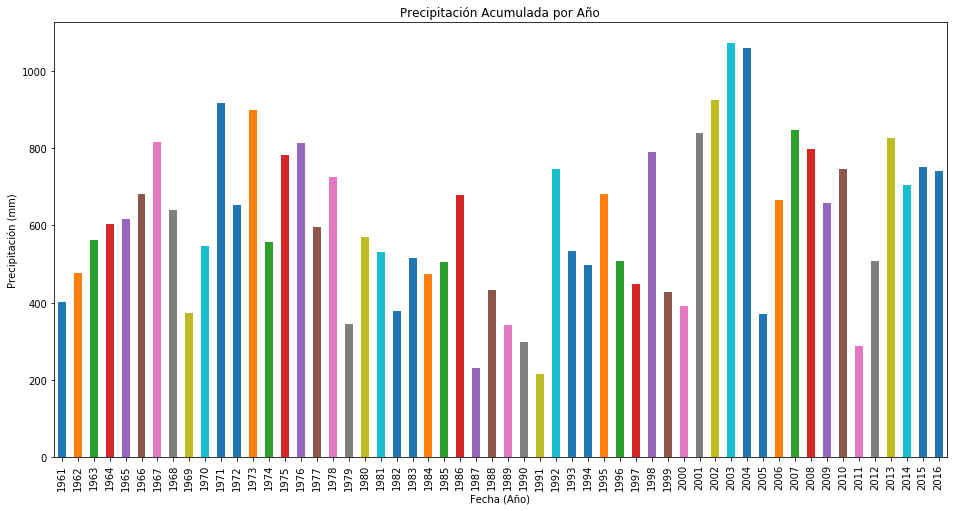
\includegraphics[scale = 0.5]{Images/PrecipY.png}
\end{center}

\subsubsection{Gráfica}
\begin{center}
    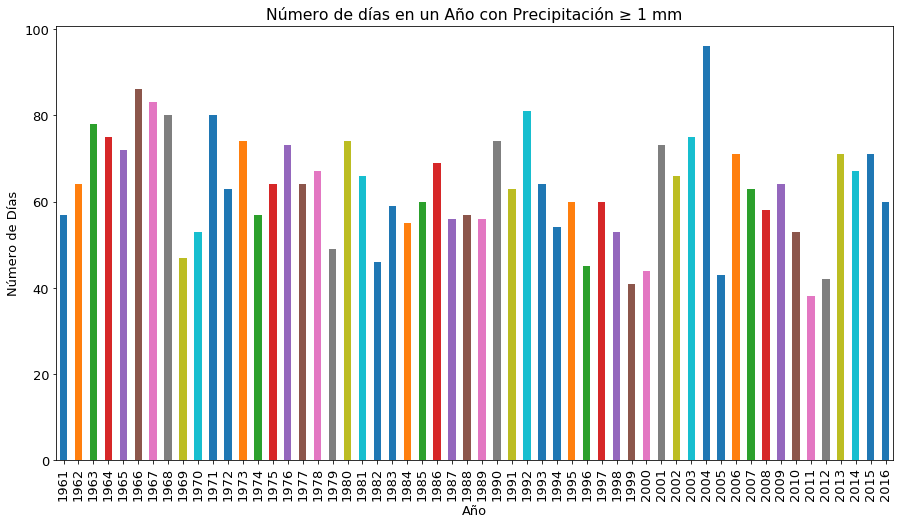
\includegraphics[width = \textwidth]{Images/GPrecipY.png}
\end{center}
Aquí vemos el número de días donde hubo precipitación mayor igual a un milímetro, donde observamos que la máxima está en el 2004, pero no se ve gran disminución de precipitaciones a años anteriores, tal vez en las últimas dos décadas sí se ha visto un poco, pero necesitaríamos ver de los últimos dos años o más para asegurar que ha habido una disminución significativa.  
\subsection{Número de Días en el Año con Precipitación Diaria Mayor Igual a 10 mm}
\subsubsection{Código}
\begin{center}
    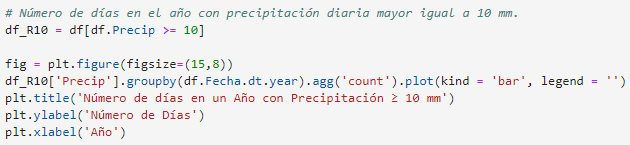
\includegraphics[scale = 0.6]{Images/PrecipY10.png}
\end{center}

\subsubsection{Gráfica}
\begin{center}
    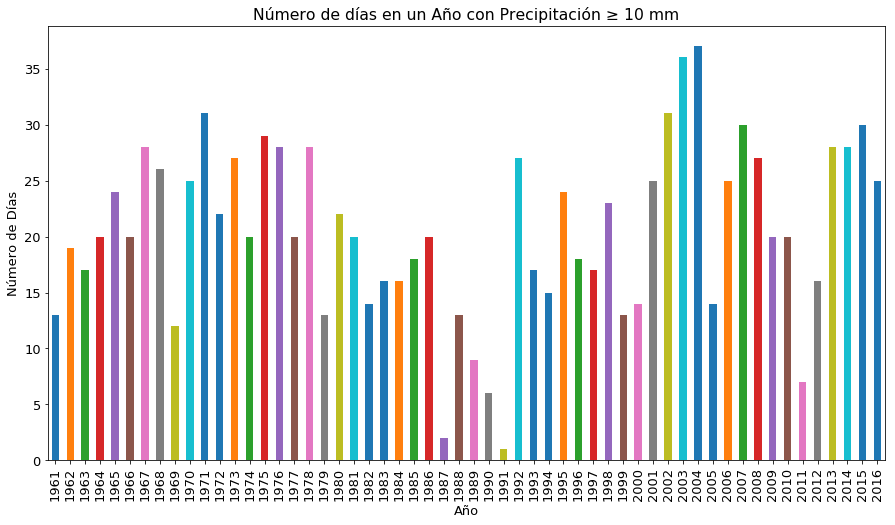
\includegraphics[width = \textwidth]{Images/GPrecipY10.png}
\end{center}
En la gráfica anterior pudimos observar que la mayoría de los años ha tenido precipitación mayor a 1 mm, pero como hablamos de cantidad, esta vez, se ve reducido el número de días con precipitación mayor igual a 10 mm, donde 1991 ha sido el más bajo hasta ahora, y el mínimo más reciente fue en el 2011.

\subsection{Número de Días en el Año con Precipitación Diaria Mayor Igual a 20mm}
\subsubsection{Código}
\begin{center}
    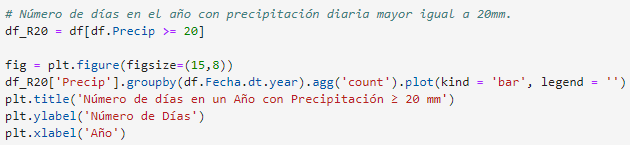
\includegraphics[scale = 0.6]{Images/PrecipY20.png}
\end{center}
\subsubsection{Gráfica}
\begin{center}
    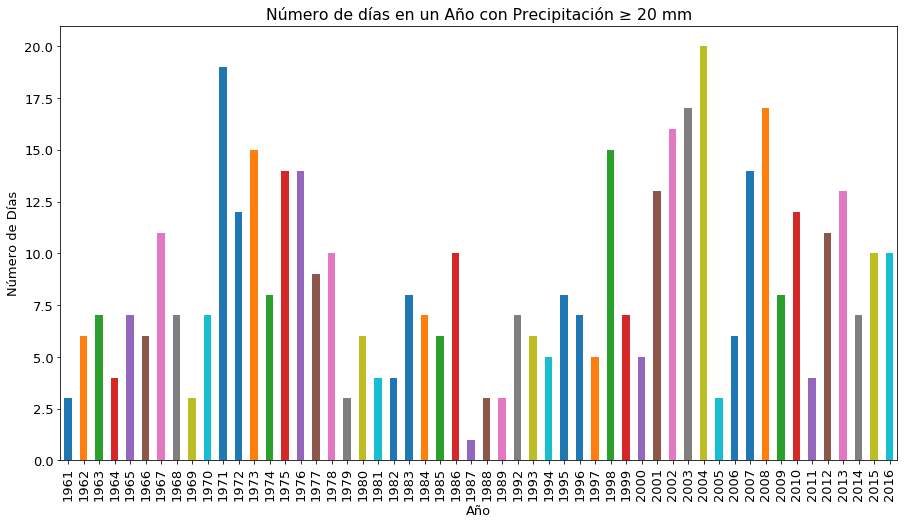
\includegraphics[width = \textwidth]{Images/GPrecipY20.png}
\end{center}
Ahora, la gráfica se ve muy diferente a la de número de días con precipitación mayor igual a 1 y 10 milímetros. En esta gráfica, ni siquiera aparece el año 1991, y el año 1987 sigue apareciendo, al parecer no hubo tantos días con precipitaciones, pero hubo gran cantidad de milímetros de precipitación.

\section{Conclusión}
\noindent Se cumplió con el objetivo principal de la actividad, la cual era seguir conociendo la librería de Matplotlib en Python, ahora obteniendo los índices del cambio climático al nivel local. También alimenta la curiosidad sobre el análisis de datos con Python y seguir buscando, por ejemplo, otros tipos de gráficos y cómo mostrar más información en una sola imagen.

En la ciudad de León no hay cambios tan bruscos o que se puedan notar fácilmente, pienso que se debe hacer un estudio más exhaustivo para encontrar irregularidades, variaciones o anomalías en el clima de León, Guanajuato. Aunque también debe ser un análisis correcto de los datos, ya que por falta de conocimiento y desarrollo en el entorno de las librerías de gráficos y código en python no se hizo un análisis completo.

Se pudieron observar muy pequeñas variaciones en los últimos años en la temperatura y precipitación, pero no fueron fáciles de encontrar. Tampoco se está siguiendo cierto tipo de patrón o algo que haga evidente el cambio climático, por lo menos en la ciudad de León.

\section{Bibliografía}
\begin{itemize}
    \item Definitions of the 27 core indices. (2009). Consultado el 24 de Febrero del 2019, de Climate Change Indices. Sitio web: 
    
    http://etccdi.pacificclimate.org/list\_27\_indices.shtml

    \item Gallery. (2019). Consultado: 15 de Febrero del 2019, de Matplotlib.org. Sitio web:
    
    https://matplotlib.org/gallery/index.html
    
    \item Matplotlib Tutorial: Python Plotting. (2017). Consultado: 15 de Febrero del 2019, de DataCamp. Sitio web: 
    
    https://www.datacamp.com/community/tutorials/matplotlib-tutorial-python
    
    \item What is Matplotlib?. (2017). Consultado: 18 de Febrero del 2019, de edureka!. Sitio web:
    
    https://www.edureka.co/blog/what-is-matplotlib/
    
    \item Boxplots. (2019). Consultado: 17 de Febrero del 2019, de Matplotlib.org. Sitio web:
    
    https://matplotlib.org/gallery/statistics/boxplot\_demo.html
    
    \item Representación gráfica de funciones y datos. (2018). Consultado: 18 de Febrero del 2019, de IAC. Sitio web: 
    
    http://www.iac.es/sieinvens/python-course/source/matplotlib.html
    
    \item Agrupación de datos por fecha en pandas. (2018). Consultado: 15 de Febrero del 2019, de Analytics Lane. Sitio web:
    
    https://www.analyticslane.com/2018/07/06/agrupacion-de-datos-por-fecha-en-pandas/
    
\end{itemize}







\end{document}
